\documentclass[10pt,a4paper]{article}
\usepackage[margin=18mm]{geometry}
\usepackage{amsmath,amssymb}
\usepackage{graphicx}
\usepackage{booktabs}
\usepackage{tikz}
\usetikzlibrary{arrows.meta}
\setlength{\parindent}{0pt}
\setlength{\parskip}{5pt}

\begin{document}

\begin{center}
  {\Large\bfseries SC4001 Neural Networks and Deep Learning}\\[5pt]
  {\large Part A: HDB Resale Price Regression}\\[5pt]
  Hu Han \quad | \quad Matriculation Number: U2320036H
\end{center}

\section*{Generative AI Declaration}
I used \textbf{Codex} to assist with the generation of selected code segments
during the development of this assignment. The tool was used primarily to
generate initial code templates and to obtain suggestions for implementing
specific programming tasks. All AI-generated code was carefully reviewed,
modified where necessary, integrated into the overall solution by me, and
tested to ensure it met the assignment requirements. I verified the correctness
of the generated code through manual inspection, compilation/execution testing,
debugging, and comparison with the assignment specifications and relevant course
materials. The final submitted work represents my own understanding and effort.
I take full responsibility for the accuracy, functionality, and academic
integrity of the submitted solution.

\textbf{Generative AI Tool Used:} Codex\\
\textbf{Purpose of Use:} Code generation and programming assistance\\
\textbf{Verification Method:} Manual code review, testing, debugging, and
validation against assignment requirements\\
\textbf{Additional uses:} Codex also assisted with report template preparation,
debugging, and interpretation of the code and assignment requirements.

\newpage
\section*{A1}
\subsection*{(a)}
\textbf{Block Diagram:}
\begin{center}
\resizebox{\linewidth}{!}{%
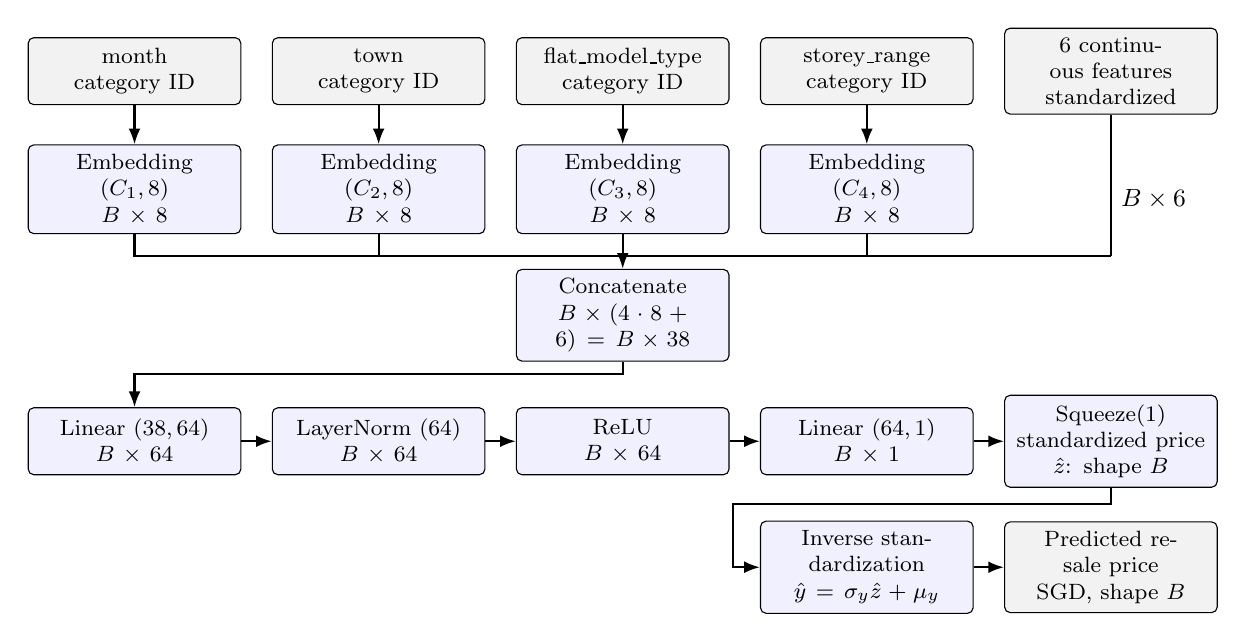
\begin{tikzpicture}[
  block/.style={draw, rounded corners=2pt, align=center,
    text width=2.45cm, minimum width=2.7cm,
    minimum height=0.85cm, font=\footnotesize},
  input/.style={block, fill=gray!10},
  layer/.style={block, fill=blue!6},
  flow/.style={-{Latex[length=2mm]}, thick}
]
  \node[input] (month) at (0,0) {month\\category ID};
  \node[input] (town) at (3.1,0) {town\\category ID};
  \node[input] (flat) at (6.2,0) {flat\_model\_type\\category ID};
  \node[input] (storey) at (9.3,0) {storey\_range\\category ID};
  \node[input] (continuous) at (12.4,0)
    {6 continuous features\\standardized};

  \node[layer] (em) at (0,-1.5) {Embedding $(C_1,8)$\\$B\times8$};
  \node[layer] (et) at (3.1,-1.5) {Embedding $(C_2,8)$\\$B\times8$};
  \node[layer] (ef) at (6.2,-1.5) {Embedding $(C_3,8)$\\$B\times8$};
  \node[layer] (es) at (9.3,-1.5) {Embedding $(C_4,8)$\\$B\times8$};
  \node[layer] (concat) at (6.2,-3.1)
    {Concatenate\\$B\times(4\cdot8+6)=B\times38$};

  \draw[flow] (month) -- (em);
  \draw[flow] (town) -- (et);
  \draw[flow] (flat) -- (ef);
  \draw[flow] (storey) -- (es);
  \draw[thick] (em.south) -- (0,-2.35) -- (12.4,-2.35);
  \draw[thick] (et.south) -- (3.1,-2.35);
  \draw[thick] (ef.south) -- (6.2,-2.35);
  \draw[thick] (es.south) -- (9.3,-2.35);
  \draw[thick] (continuous.south) -- (12.4,-2.35)
    node[pos=0.6,right,font=\small] {$B\times6$};
  \draw[flow] (6.2,-2.35) -- (concat.north);

  \node[layer] (linear1) at (0,-4.7) {Linear $(38,64)$\\$B\times64$};
  \node[layer] (norm) at (3.1,-4.7) {LayerNorm $(64)$\\$B\times64$};
  \node[layer] (relu) at (6.2,-4.7) {ReLU\\$B\times64$};
  \node[layer] (linear2) at (9.3,-4.7) {Linear $(64,1)$\\$B\times1$};
  \node[layer] (standard) at (12.4,-4.7)
    {Squeeze(1)\\standardized price\\$\hat z$: shape $B$};
  \draw[flow] (concat.south) -- (6.2,-3.85) -- (0,-3.85)
    -- (linear1.north);
  \draw[flow] (linear1) -- (norm);
  \draw[flow] (norm) -- (relu);
  \draw[flow] (relu) -- (linear2);
  \draw[flow] (linear2) -- (standard);

  \node[layer] (inverse) at (9.3,-6.3)
    {Inverse standardization\\$\hat y=\sigma_y\hat z+\mu_y$};
  \node[input] (output) at (12.4,-6.3)
    {Predicted resale price\\SGD, shape $B$};
  \draw[flow] (standard.south) -- (12.4,-5.5) -- (7.6,-5.5)
    -- (7.6,-6.3) -- (inverse.west);
  \draw[flow] (inverse) -- (output);
\end{tikzpicture}%
}
\end{center}

Explanation:

\begin{itemize}
  \setlength{\itemsep}{0pt}
  \setlength{\parskip}{0pt}
  \item Each categorical embedding has dimension 8.
  \item The hidden layer has width 64.
  \item $B$ denotes the batch size.
  \item $C_j$ counts the known training categories for feature $j$, plus one
    extra category with ID 0 for unknown values.
\end{itemize}

\textbf{Number of trainable parameters:}

Each categorical feature $j$ uses an embedding table with $C_j$ rows and 8
trainable values per row. We add one extra category for unknown category for each feature, which gives:
\[
C_j = \text{number of categories in feature } j + 1.
\]

Calculate $C_j$ for every categorical features:

\begin{center}
\begin{tabular}{lrc}
\toprule
Categorical feature & Number of training categories & $C_j$ calculation\\
\midrule
\texttt{month} & 12 & $C_1=12+1=13$\\
\texttt{town} & 26 & $C_2=26+1=27$\\
\texttt{flat\_model\_type} & 43 & $C_3=43+1=44$\\
\texttt{storey\_range} & 17 & $C_4=17+1=18$\\
\bottomrule
\end{tabular}
\end{center}

Six continuous features: \texttt{dist\_to\_nearest\_stn},
\texttt{dist\_to\_dhoby}, \texttt{degree\_centrality},
\texttt{eigenvector\_centrality}, \texttt{remaining\_lease\_years}, and
\texttt{floor\_area\_sqm}. 

Each contributes one input value. Concatenating the four 8-dimensional embeddings with these six values gives the total input dimension $D$:
\[
  D=4\times8+6=38.
\]
Layer-by-layer trainable parameter counts:

\begin{center}
\begin{tabular}{lrr}
\toprule
Component & Calculation & Trainable parameters\\
\midrule
Four embedding tables & $(13+27+44+18)\times8$ & 816\\
Linear $(38,64)$ & $38\times64+64$ & 2,496\\
LayerNorm $(64)$ & $64+64$ & 128\\
Linear $(64,1)$ & $64\times1+1$ & 65\\
\midrule
\textbf{Total} & $816+2{,}496+128+65$ & \textbf{3,505}\\
\bottomrule
\end{tabular}
\end{center}

Explanation:

\begin{itemize}
\item Each linear layer includes a weight matrix and a bias vector. 
\item LayerNorm has 64 learnable scale parameters and 64 learnable shift parameters. 
\item Concatenation, ReLU, squeezing, and inverse target standardization add no trainable parameters.
\end{itemize}

\subsection*{(b)}

\subsection*{(c)}

\subsection*{(d)}

\subsection*{(e)}

\section*{A2}

\section*{A3}

\section*{A4}

\end{document}
